\documentclass{article}
\usepackage[numbers,sort&compress]{natbib}
\usepackage{graphicx}
\usepackage{amsmath}
\usepackage{amssymb}
\usepackage{bm}
\usepackage{color}
\begin{document}
\begin{abstract}
Recently we investigated the applicability and parameters choice for the two-dimensional case
Bretherton problem using the lattice Boltzmann method (LBM) {\color{red} Give citation here}. This
paper is the continuation of the previous work and is focused on the three-dimensional case to
validate the LBM for simulation of phenomena for rectangular and square capillaries in the
moderate range of Capillary number parameters. 
\end{abstract}
\section{What to examine}
I suggest to examine first of all the application of the LBM for really small capillary number,
where it's not possible to resolve the interface. In this case one should find the asymmetric
radiuses for the droplet, the difference should be around $10$ percent. While applying the forcing
it should come to the spheric shape. As well we need to examine the capillary number dependancy on
the length and suggest to examine some axicentric factors for rectangular channels.

\section{Introduction}
While for two-dimensional Bretherton flow the results are usually limited to the circular shape and
only some of them are for the plane-symmetric case \cite{giavedoni-numerical,heil-bretherton},
vast number of experimental results and simulations are available for the three-dimensional case.
It was found that the for rectangular and/or square shaped capillaries there is a transition for
certain capillary number, where the flow changes from the non axisymmetric to axis symmetric case.
The number is indicated in a number of works of as $\hat{Ca}=0.04$ \cite{cerro-bubble-train},
$\hat{Ca}=0.1$
\cite{cerro-space}, $\hat{Ca}=0.033$ \cite{heil-threedim}. If the capillary number is larger than
the critical capillary number, i.e. $Ca>\hat{Ca}$, then the flow becomes axisimmetric with the
radius of the droplet dependant on the capillary number.

The following pictures summarize the radius of deposited liquid on the capillary length.
\citet{heil-threedim} performed three-dimensional simulations for circular shaped and for the
square shaped capillaries and gravitational effects for circular shaped capillaries. The results for
square capillaries are shown in Fig.\ref{fig:heil:three:dim}. On another hand authors performed
numerical simulations for rectangular shaped capillaries. It was found that aspect ratio $\alpha$
allows to put all the different curves on one purely empirical curve through the following parameter
$s_{\infty}=r_{\infty} \alpha^{-1/2}$, where $r_{\infty}$ is the aximsymmetric bubble radius
infinitely far behind the bubble tip and can be calculated from the flow rate in the computational
domain:
\begin{equation}
r_{\infty}=2\sqrt{(a-Q)/\pi}.
\end{equation}
It is also indicated that for $\alpha\geq\hat{\alpha}=2.04$ the interface can not make up the
axisymmetric case. The $s_{\infty}$ dependency on $\alpha$ is shown in Fig.
\ref{fig:heil:three:dim}.
\begin{figure}
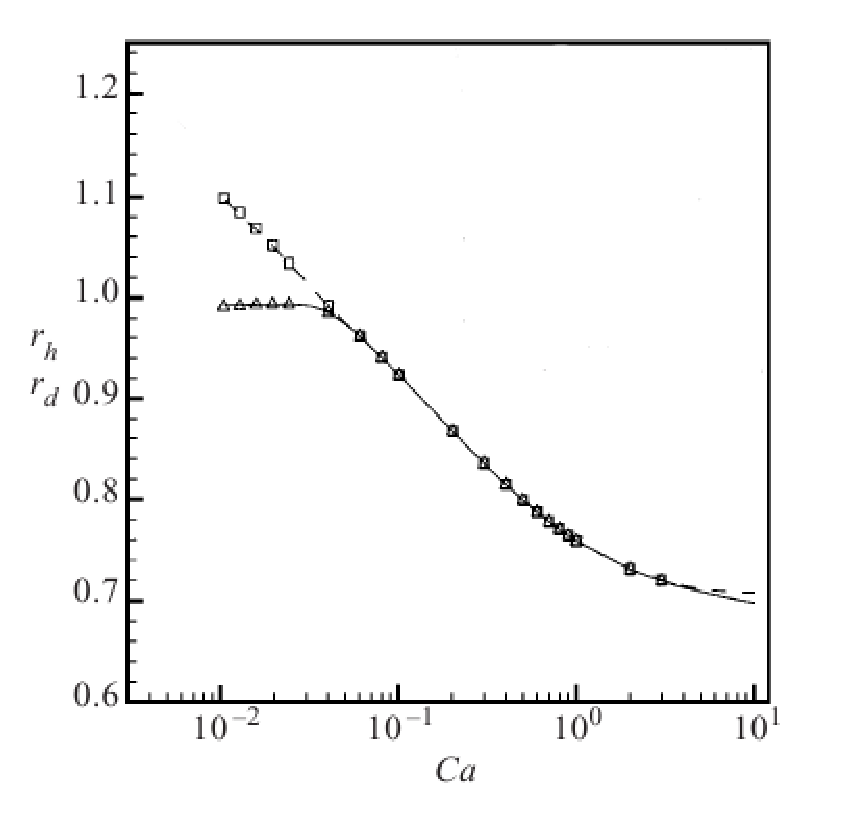
\includegraphics[width=0.47\textwidth]{Figures/capillary_width_heil.eps}\hfill
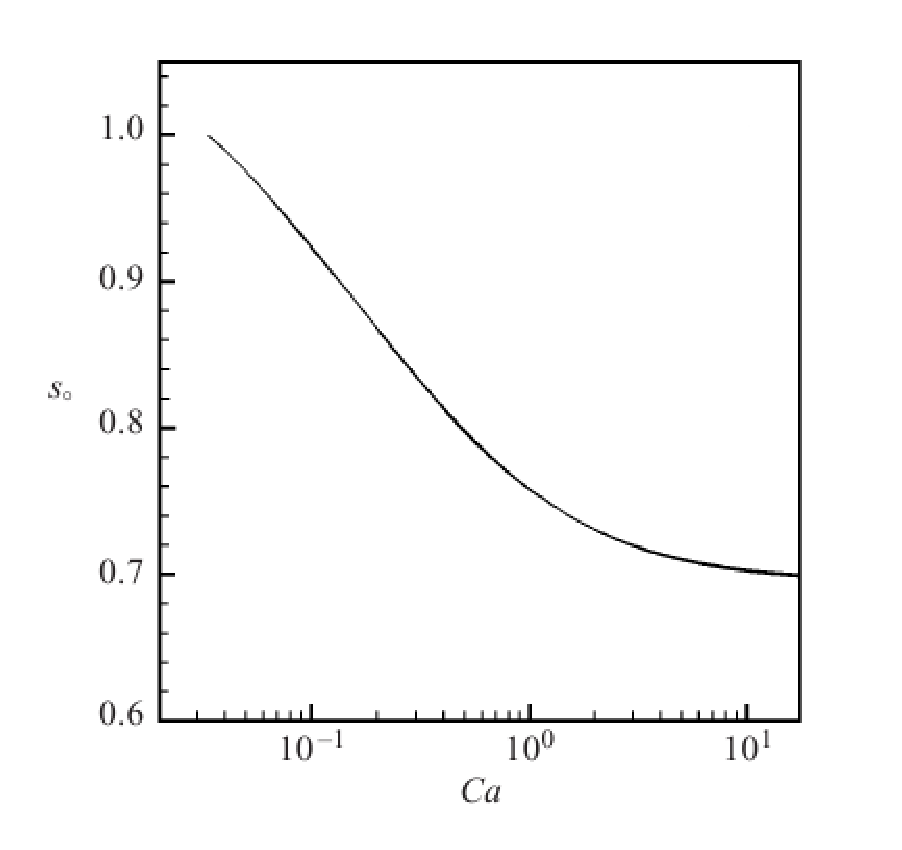
\includegraphics[width=0.47\textwidth]{Figures/capillary_rectangular_width_heil.eps}\\
\caption{\citet{heil-threedim} results for the variation of the deposited liquid for the range of
capillary number. One can see the asymmetry between diagonal and axis diameter for the capillary
number $Ca\leq\hat{Ca}=0.04$.\label{fig:heil:three:dim}}
\end{figure}
There is also interesting thing to track down is the recirculating regime for flow fields. It is
known that for certain capillary number the streamlines either go around the bubble or create the
circulating regime in front of the bubble. The calculation ({\color{red} or analytical data? Look
at White 1991, pp. 119-120. As well put figures if there is a space from Heil et al.}) are presented
in Table \ref{table:recirculation:data}.
\begin{table}
\begin{tabular}{c|c}
$\alpha$& $Ca_{T}$\\
\hline
1& 0.691\\
1.1 & 0.688\\
1.3 & 0.666\\
1.5 & 0.631\\
\end{tabular}
\caption{The results for the recirculation region.\label{table:recirculation:data}}
\end{table}

\citet{shikazono-square} obtained a lot of different results for the deposition length versus the
capillary number variation for FC-40/air, ethanol/air and water/air experiments. All of them are
presented in Fig. \ref{fig:deposition:han}.
\begin{figure}
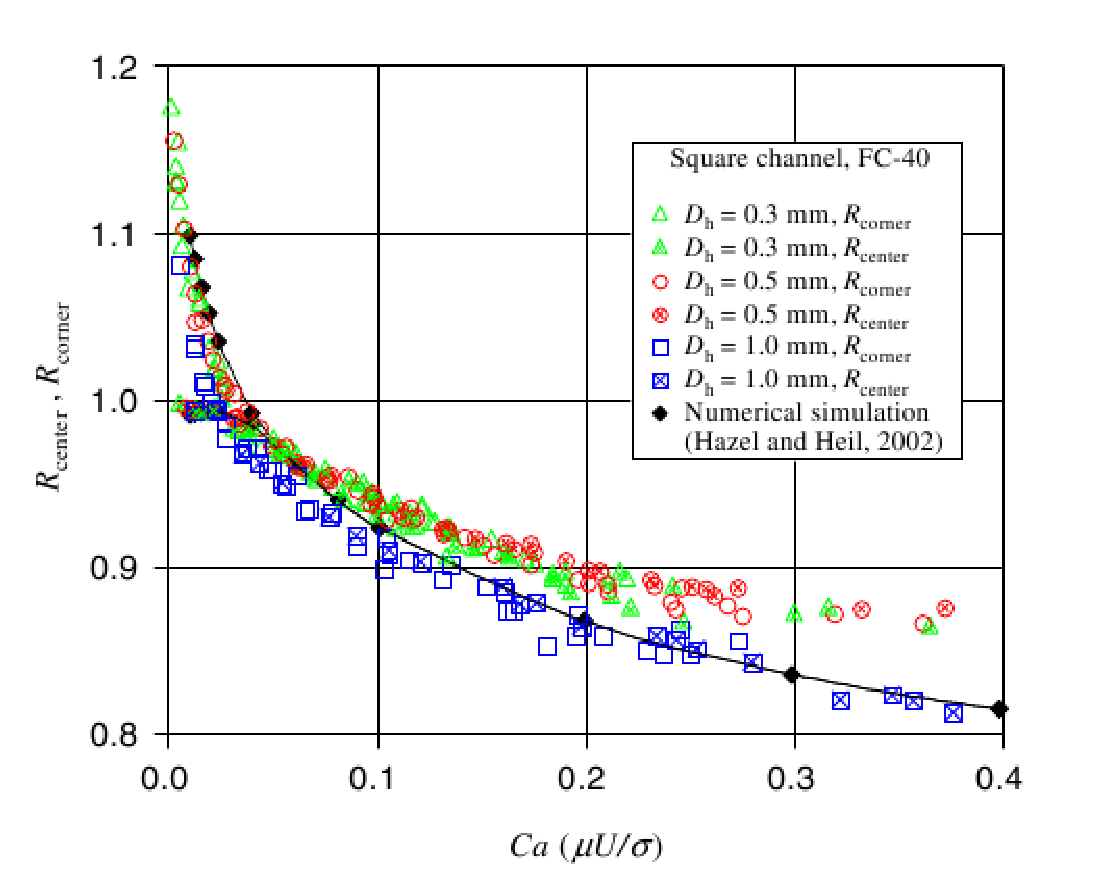
\includegraphics[width=0.33\textwidth]{Figures/han_capillary_fc40_air.eps}\hfill
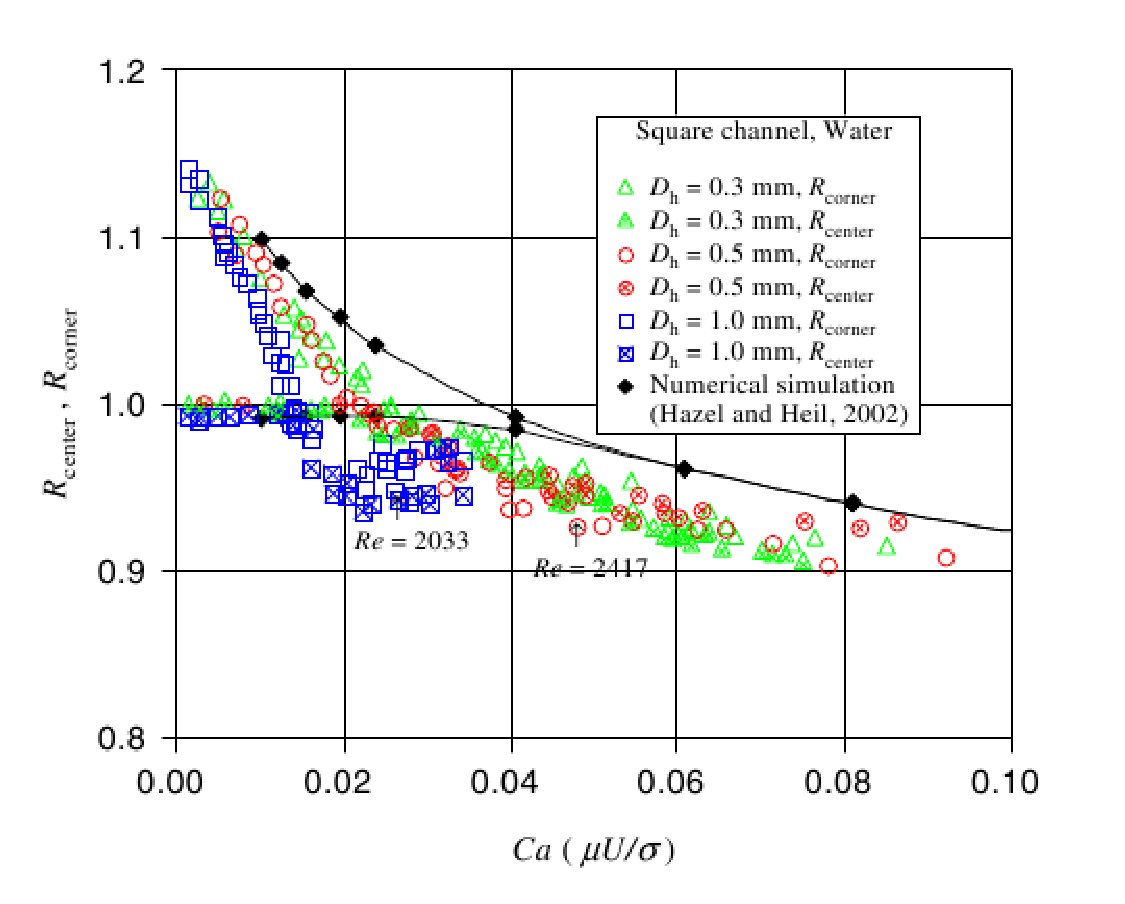
\includegraphics[width=0.33\textwidth]{Figures/han_capillary_water_air.eps}\hfill
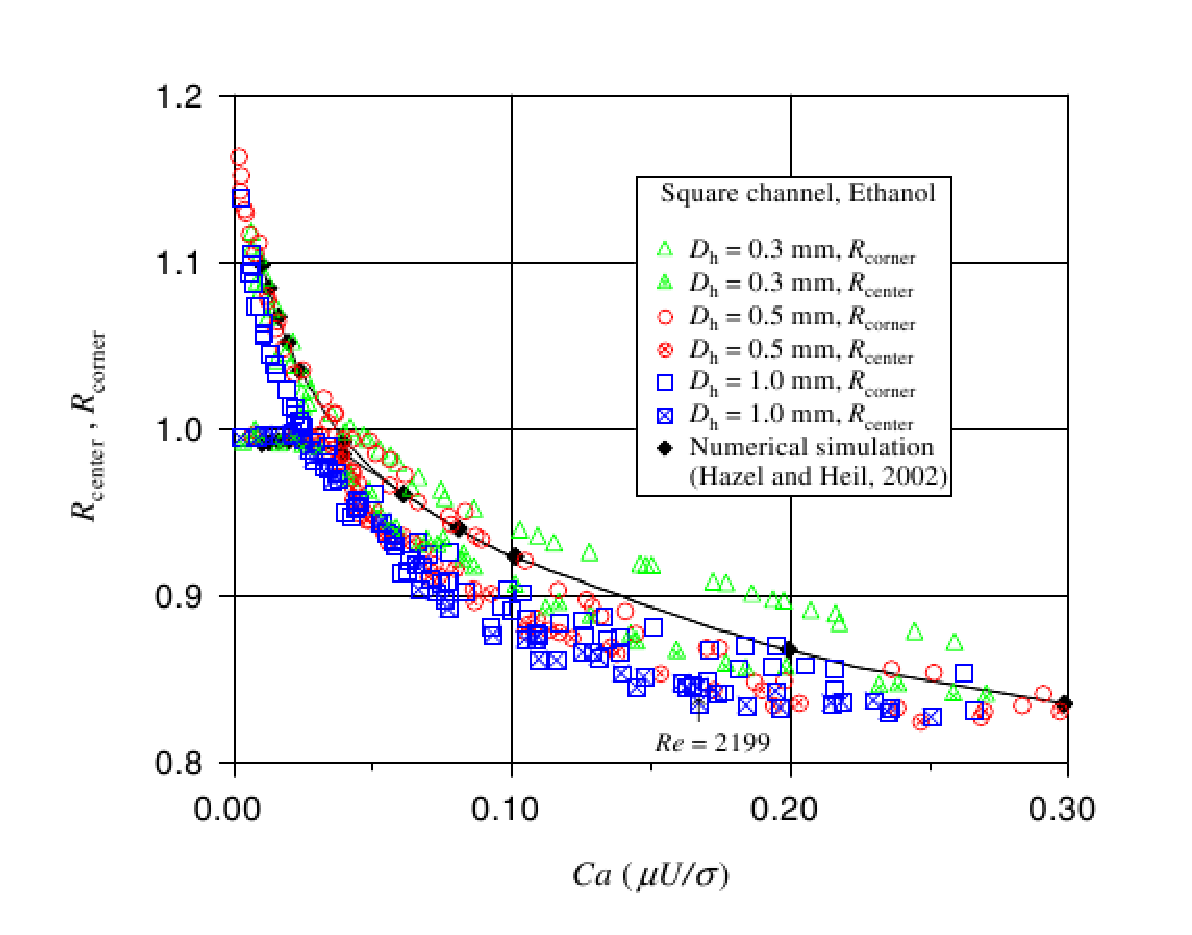
\includegraphics[width=0.33\textwidth]{Figures/han_capillary_ethanol_air.eps}\\
\caption{Han results. \label{fig:deposition:han}}
\end{figure}

\citet{cerro-bubble-train} performed a lot of experiments for a buble-train flow in capillaries of
circular and square cross section for horizontal, upward and downward flows. The main results are
presented in Fig. \ref{fig:thulasidas:results}.
\begin{figure}
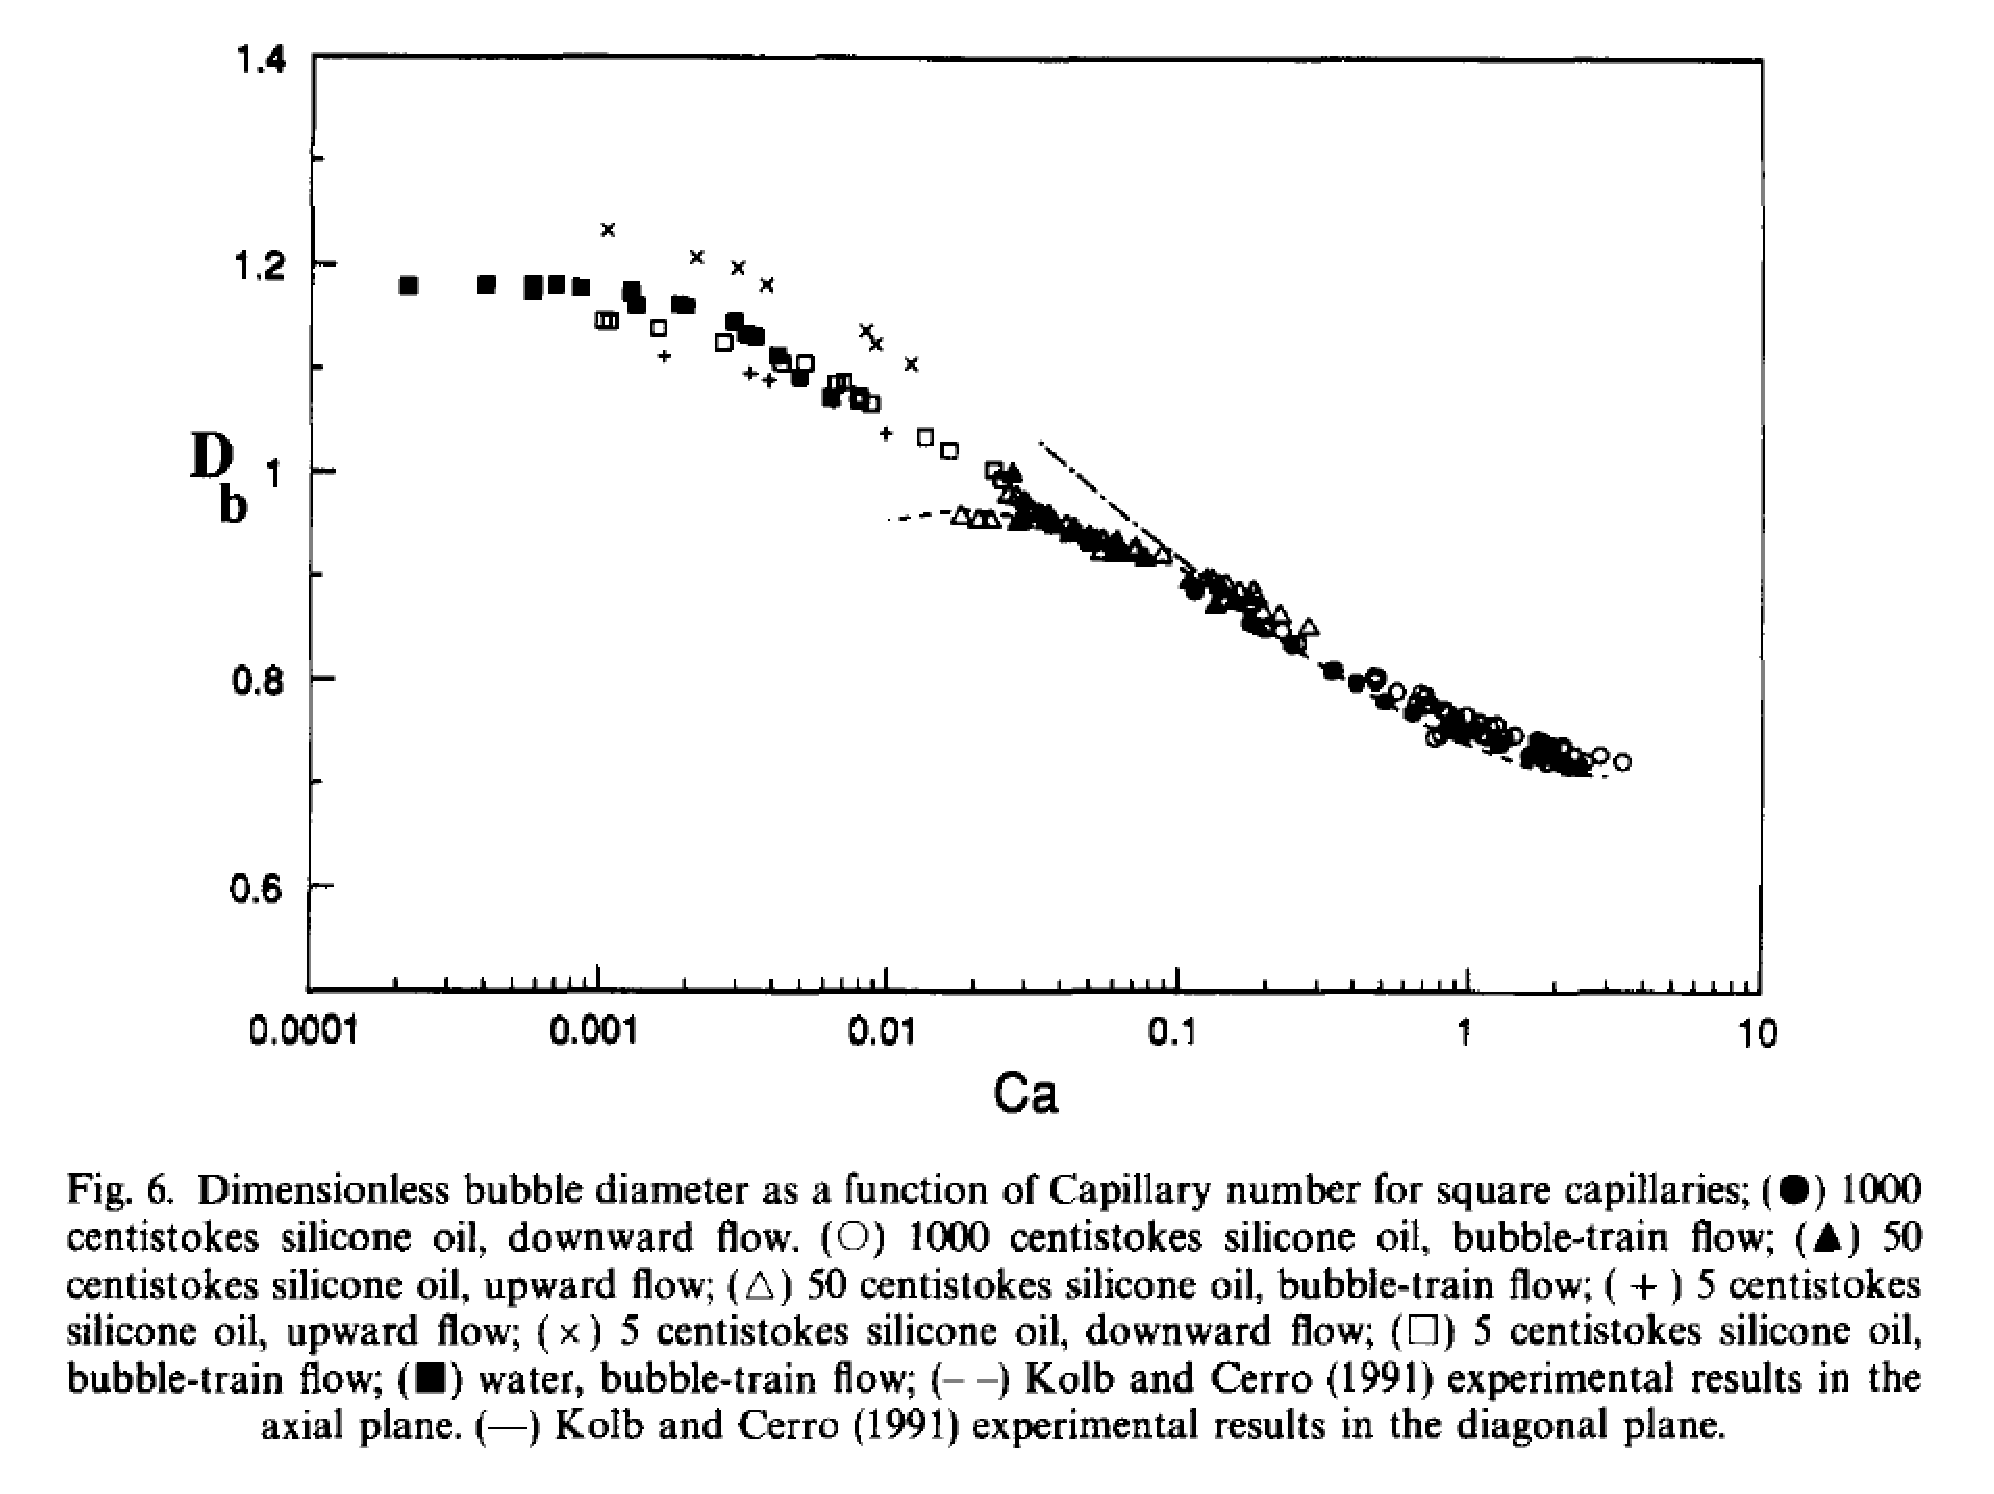
\includegraphics[width=0.47\textwidth]{Figures/thulasidas_capillary.eps}\hfill
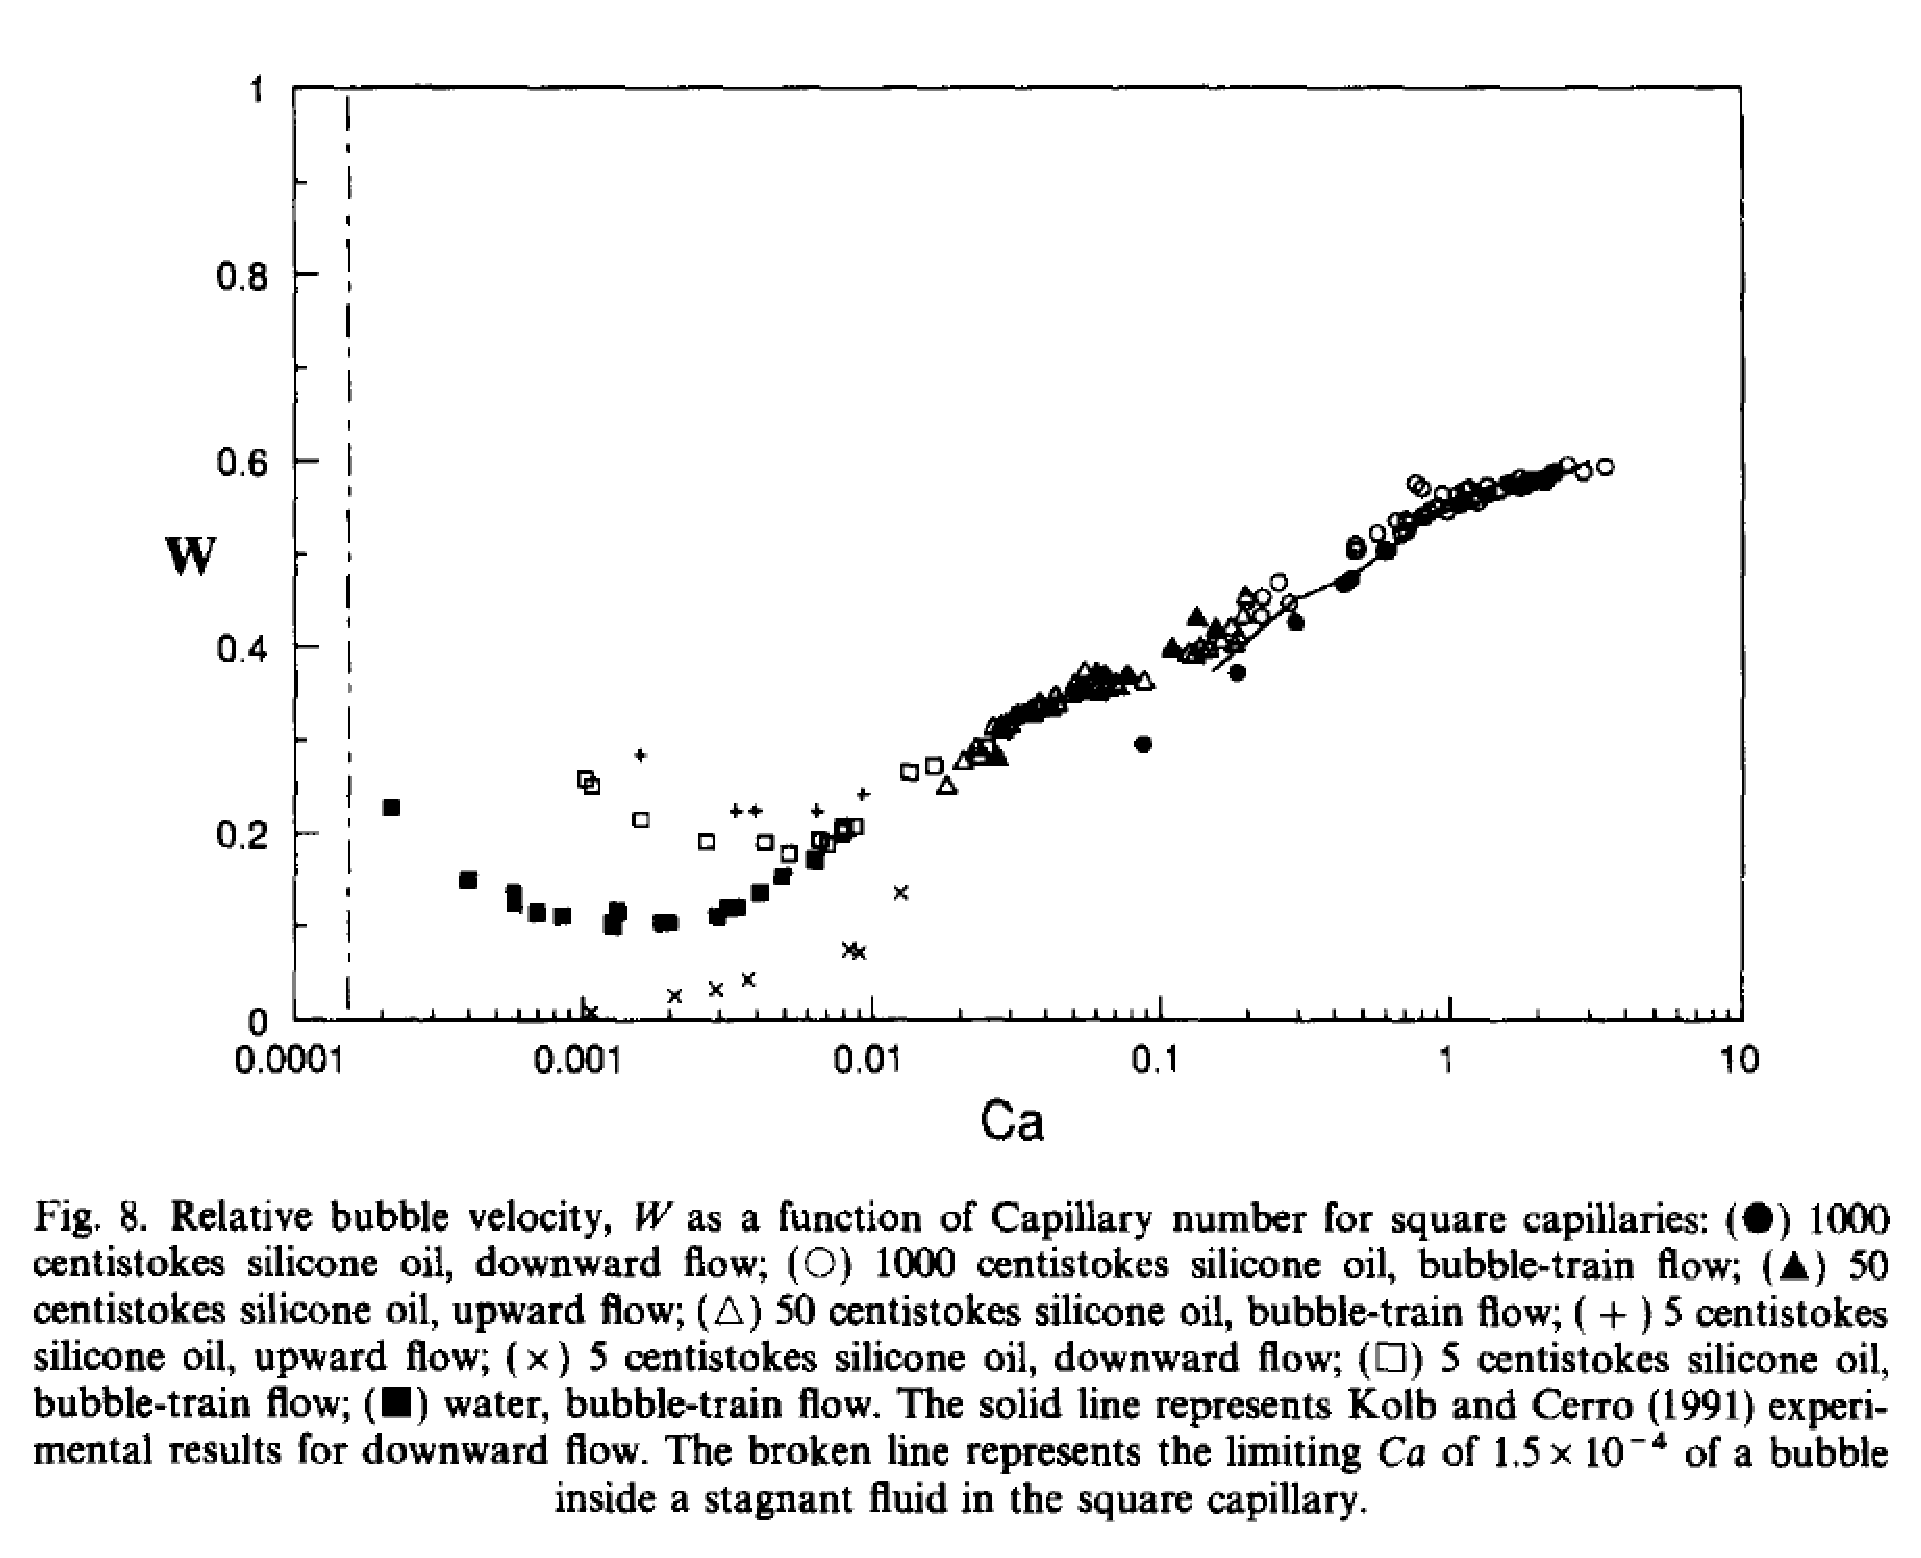
\includegraphics[width=0.47\textwidth]{Figures/thulasidas_relative_velocity.eps}\\
\caption{\citet{cerro-bubble-train} results for the film thickness
variation and the relative bubble velocity versus the capillary
number.\label{fig:thulasidas:results}}
\end{figure}

\citet{wang-non-circular} performed numerical simulations by VOF technique to for the non-circular
shaped capillaries as square and triangle shaped capillaries. Some interesting results for bubble
shape depending on the capillary number, Fig. \ref{fig:wang:bubble:shape}. They also included
numerical simulations for the determination of the critical capillary number $\hat{Ca}$, Fig.
\ref{fig:wang:critical:capillary}. They also found the relative velocity for the bubble for
different capillary numbers. \ref{fig:wang:critical:capillary}.
\begin{figure}
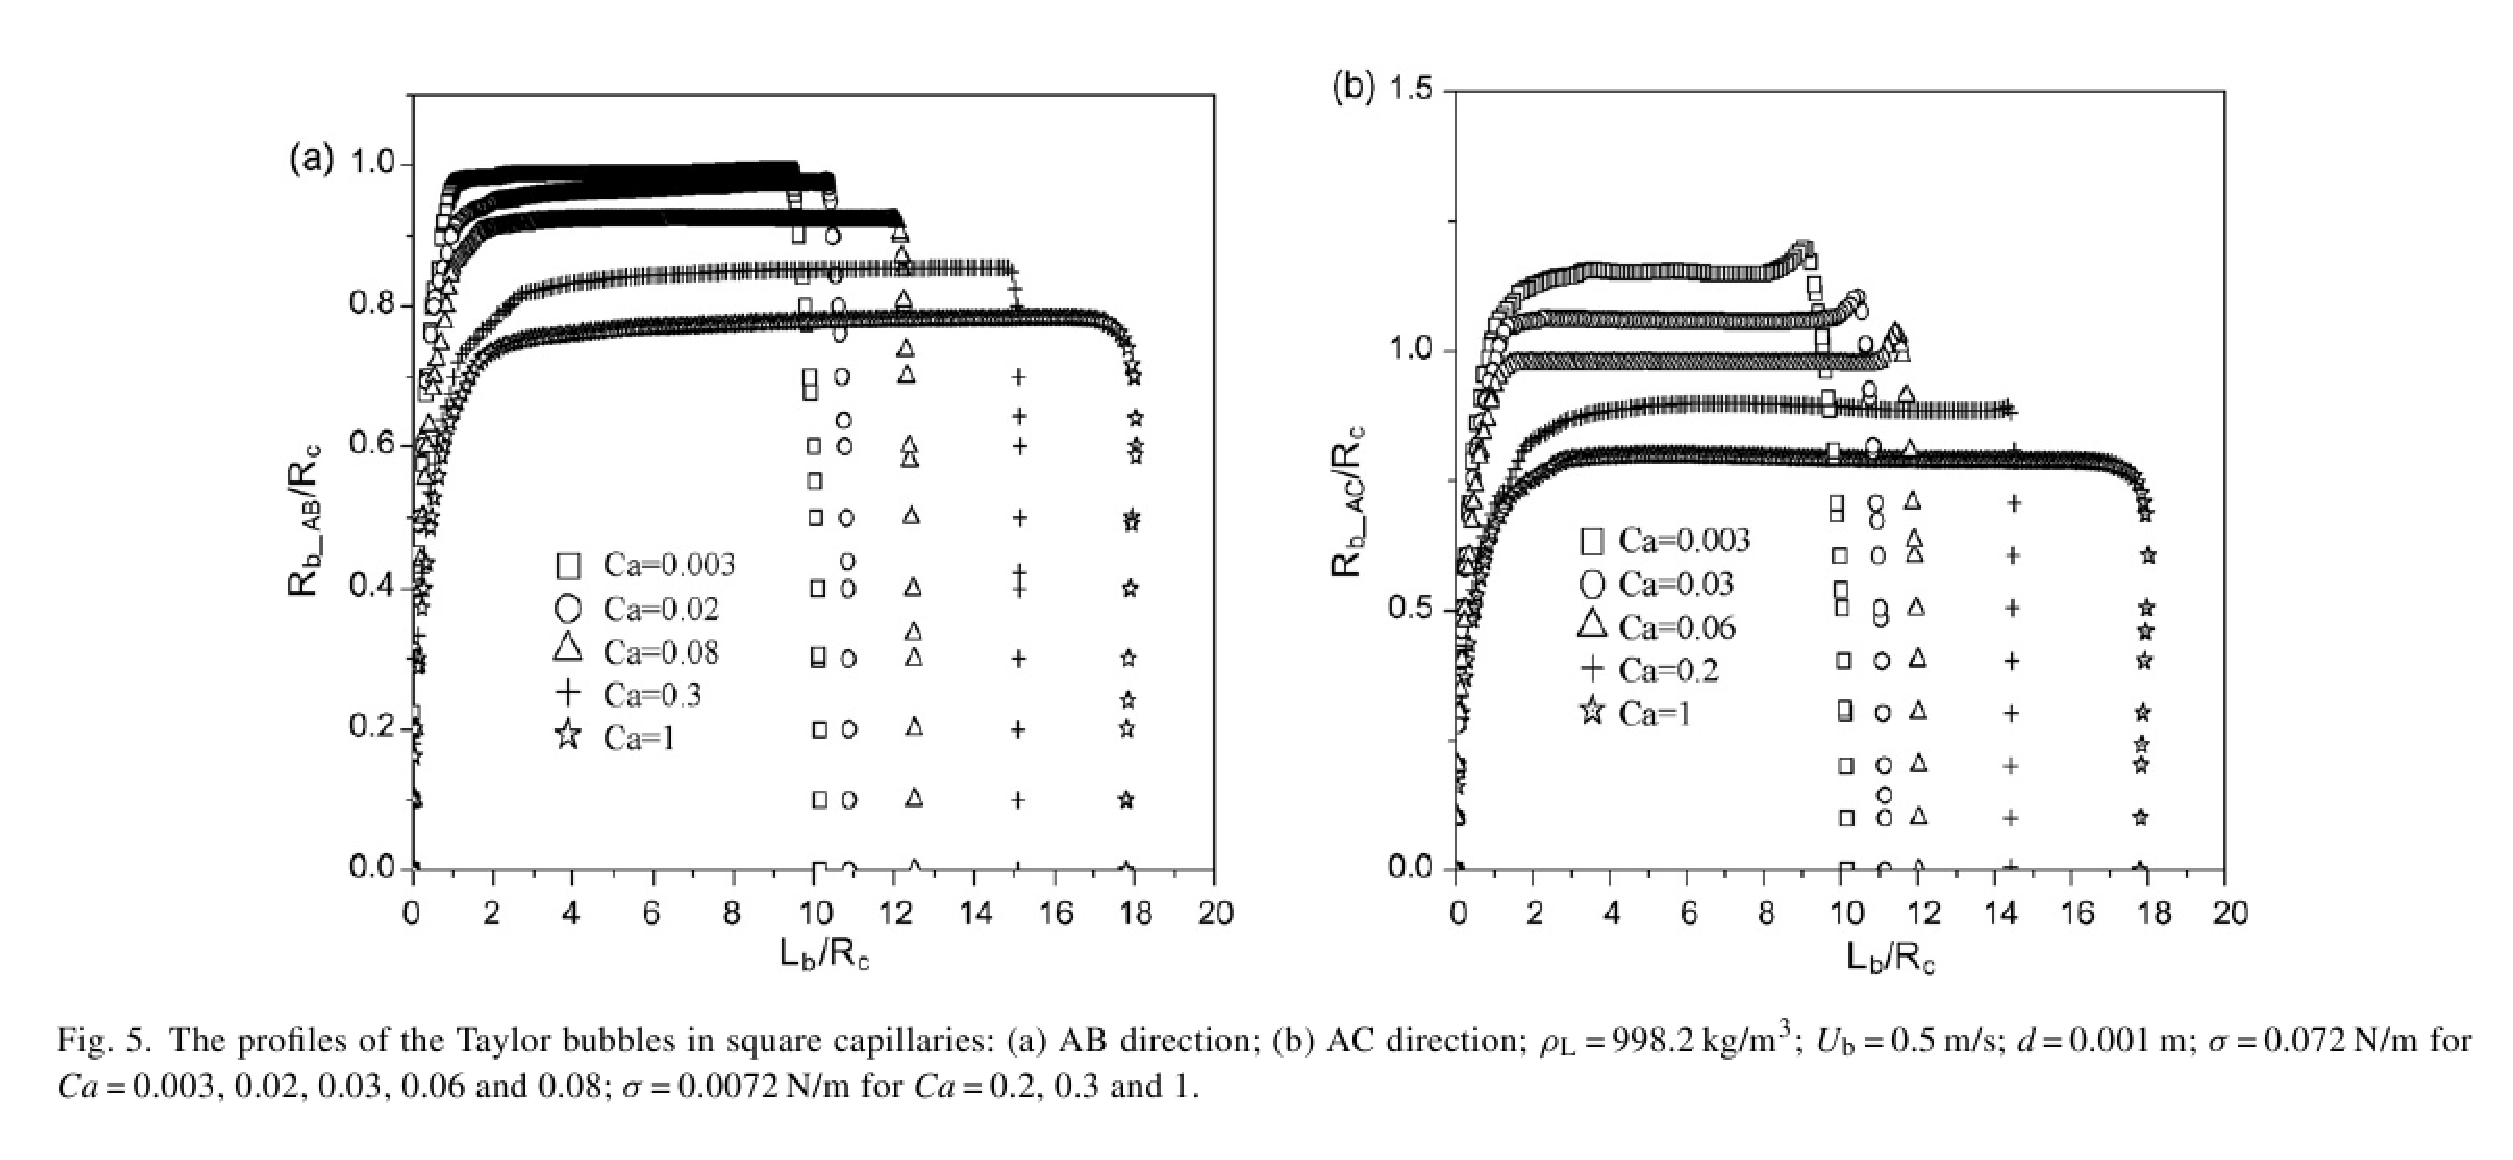
\includegraphics[width=\textwidth]{Figures/wang_bubble_shape.eps}
\caption{The bubble shape across the length for different capillary numbers.
\label{fig:wang:bubble:shape}}
\end{figure}
\begin{figure}
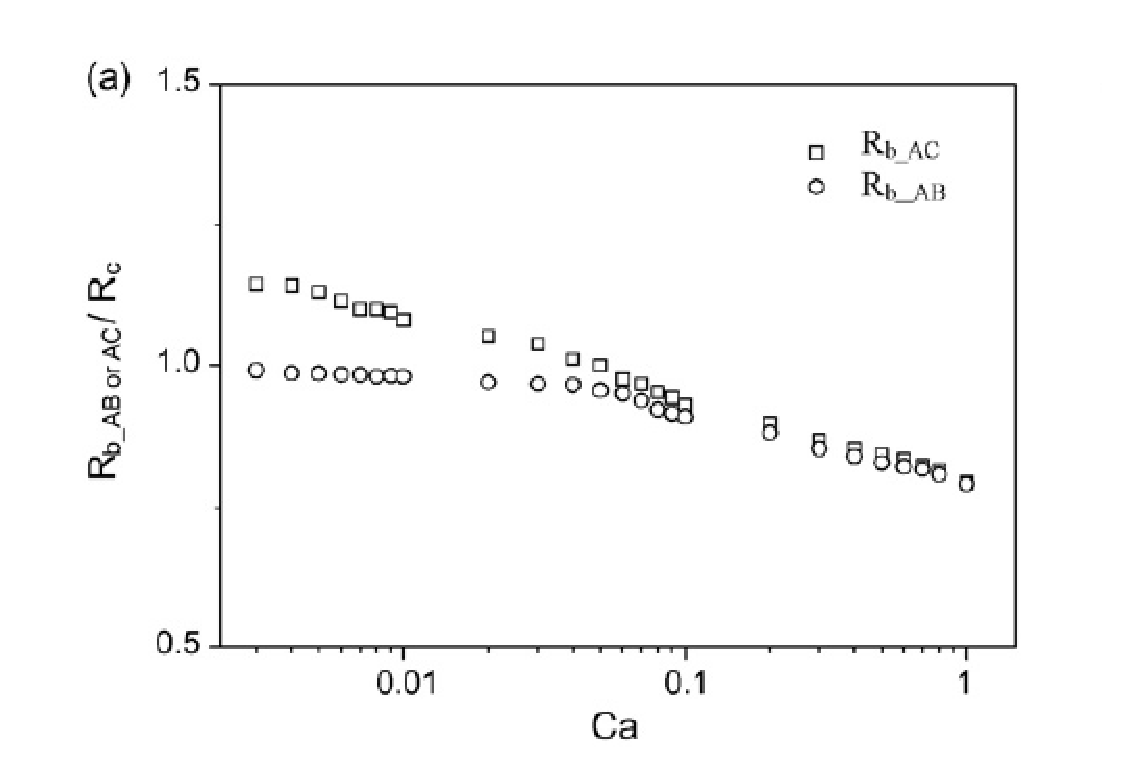
\includegraphics[width=0.47\textwidth]{Figures/wang_critical_capillary.eps}\hfill
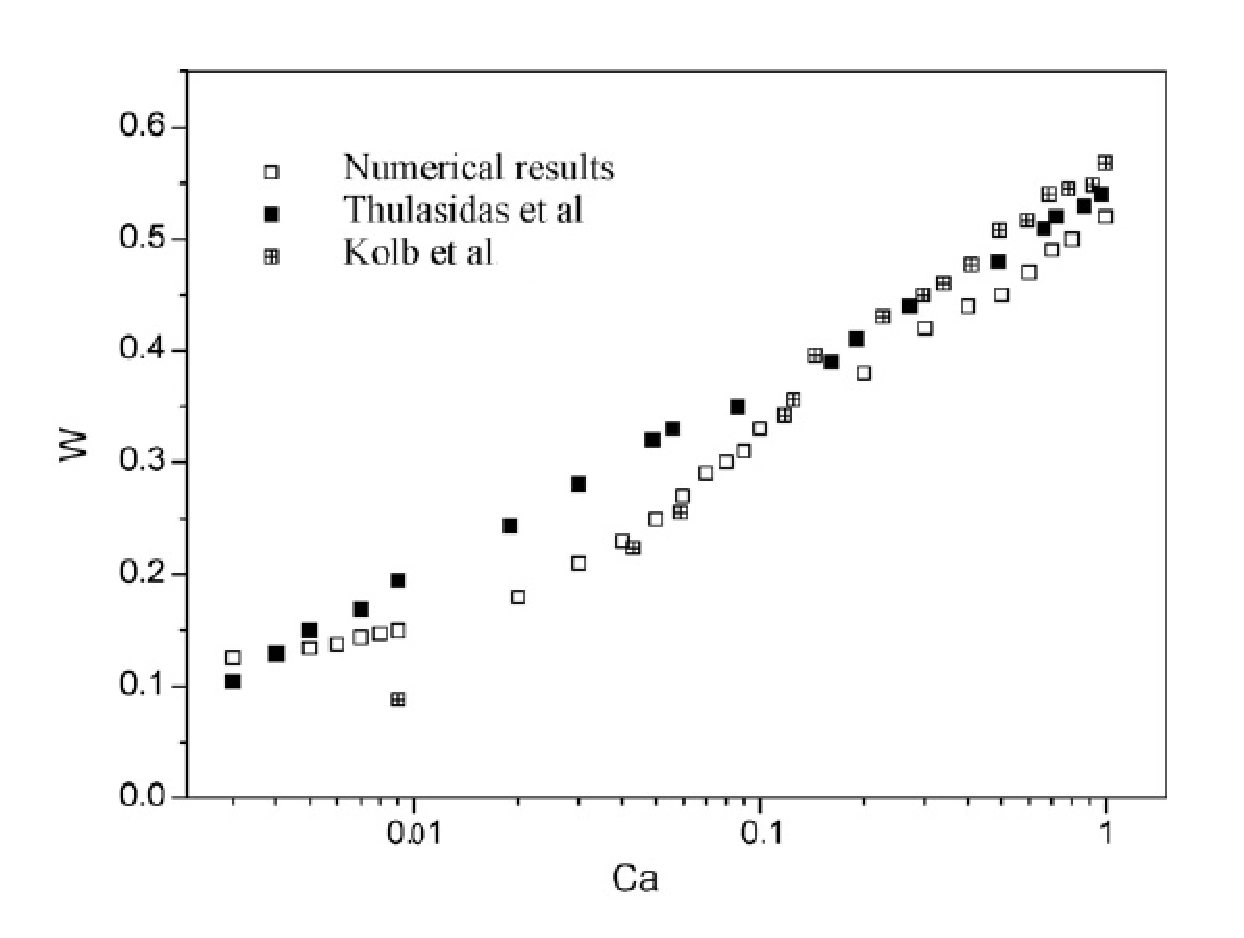
\includegraphics[width=0.47\textwidth]{Figures/wang_relative_velocity.eps}
\caption{Bubble radiuses variations over the range of capillary numbers (left) and the relative
velocity depending on the capillary number  \label{fig:wang:critical:capillary}}
\end{figure}


\section{Variation bubble length}
The work of \cite{heil-threedim} shows the variation of the bubble thickness through the length of
bubble. The length variation is presented in Fig. \ref{fig:thickness:variation:ca:ten}
\begin{figure}
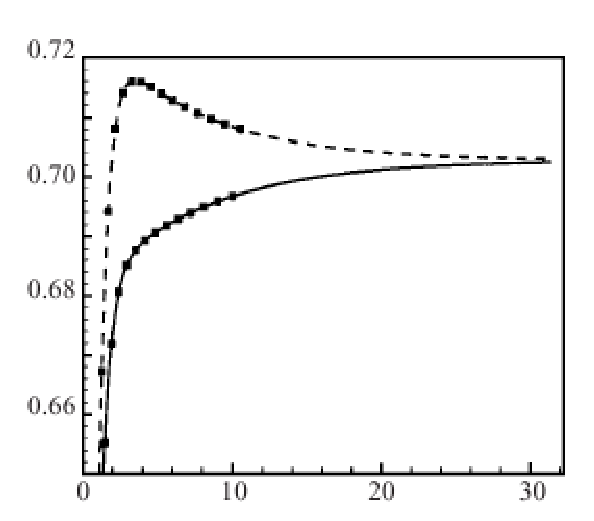
\includegraphics[width=0.97\textwidth]{Figures/variationoverlength.eps}
\caption{The variation of the bubble length for capillary number $Ca=10$. The x-axis scaled to
half-width of the microchannel height.  \label{fig:thickness:variation:ca:ten}}
\end{figure}
We want to obtain the same characteristics as indicated in Fig.
\ref{fig:thickness:variation:ca:ten}. One can see that the difference between diagonal radius and
usual radius is of order of $4\%$. That means it's 2 percent of the channel height. If the
simulation is conducted by the grid $50\mathrm{x}50$ in the cross section that means that we will
see the difference in one grid node. Therefore the grid is $52\mathrm{x}52\mathrm{750}$. Here we
conduct a scaling:
\begin{equation}
Ca=\frac{\mu_{liq} U_{bubble}}{\gamma}
\end{equation}
The parameters for the binary liquid problem are chosen as $A=0.04$ and $k=0.01$. Therefore the
surface tension is:
\begin{equation}
\sigma = \sqrt{\frac{8 k A}{9}}=0.0596
\end{equation}
The relaxation times for liquid and gas are taken as, $\tau_{gas}=0.7$ and $\tau_{liq}=2.5$,
therefore the viscosities ratio is $10$.
\begin{equation}
\begin{aligned}
&10=\frac{\frac{2}{3} U_{bubble}}{0.0596},
&U_{bubble}=0.894
\end{aligned}
\end{equation}
which is quite high for the lattice Boltzmann method. We can decrease the ratio by scaling
parameters $k$ and $A$ while keeping the interface thickness. Let us choose parameters as $k=0.001$
and $A=0.004$, therefore the mobility should be adjusted to address the issue with small parameters
and small surface tension in this case. It parameters are chosen as $A=0.004$ and $k=0.001$ then
the velocity of the bubble is  $0.0894$. Therefore we can adjust the pressure gradient to plug it
into the bubble initialization:
\begin{equation}
\frac{\mathrm{d}P}{\mathrm{d}x}=\frac{8}{N_y^2} \gamma Ca=0.0001907,
\end{equation}
which is quite high for lattice Boltzmann simulations. Therefore probably one more time the surface
tension needs to be reduced. {\color{red} Many authors state that increasing mobility kills the
proper results of simulations}. 
The film thickness as it is seen from the picture is taken as $70$ percent of the half channel.
Therefore the initalization width is $0.15*50=7.5$. 

\section{Non-axisymmetric case}
For example according to \cite{heil-threedim} for the capillary
number $Ca=0.01$, the radiuses converge as $r_h=0.99$ and $r_d=1.1$. Therefore one needs to resolve
as the $0.5\%$ of whole channel width to see the difference. That certainly implies so large grid
that can kill the simulation at least $200x200x3000$. However, we can refer to artificially made
interface as $1-2$ lattice Boltzmann units but keeping the capillary number as it is required. In
this case we can refer like we can't resolve the interface. However, one can check whether
completely underresolved interfaces can give something good with the continuous interface methods.
The dimensionalization case is therefore as follows. Instead of starting with the capillary number
simulations we initialize the initial thickness with $2.5$ lattice boltzmann units, change the
pressure gradients through the following numbers:
\begin{equation}
\frac{\mathrm{d}P}{\mathrm{d}x}=
\begin{cases}
1\dots10\mathrm{x}10^{-6}\\
10,15\dots 100 \mathrm{x}10^{-6}
\end{cases}
\end{equation}
After performing the simulations we determine the $R_{axis}$, $R_{diag}$ versus calculated
capillary number
\begin{equation}
Ca=\frac{\mu_{liq} U_{bubble}}{\gamma}.
\end{equation}
To perform simulations we
started with the following parameters as
$k=0.04$,$A=0.04$,$\Gamma=1.0$,$N_x\mathrm{x}N_y\mathrm{x}N_z=52\mathrm{x}52\mathrm{x}750$.
For underresolved schemes, the pressure gradient doesn't work in the way we expect. Therefore, we
take pressure gradient in the following way and later on establish the associated capillary number.
We want to keep track of $R_{diag}$ when the $R_{axis}$ is underresolved. The preliminary results
for the film thickness measured in the middle of the bubble are shown in Fig.
\ref{fig:underresolved:capillaries}. 
\begin{figure}
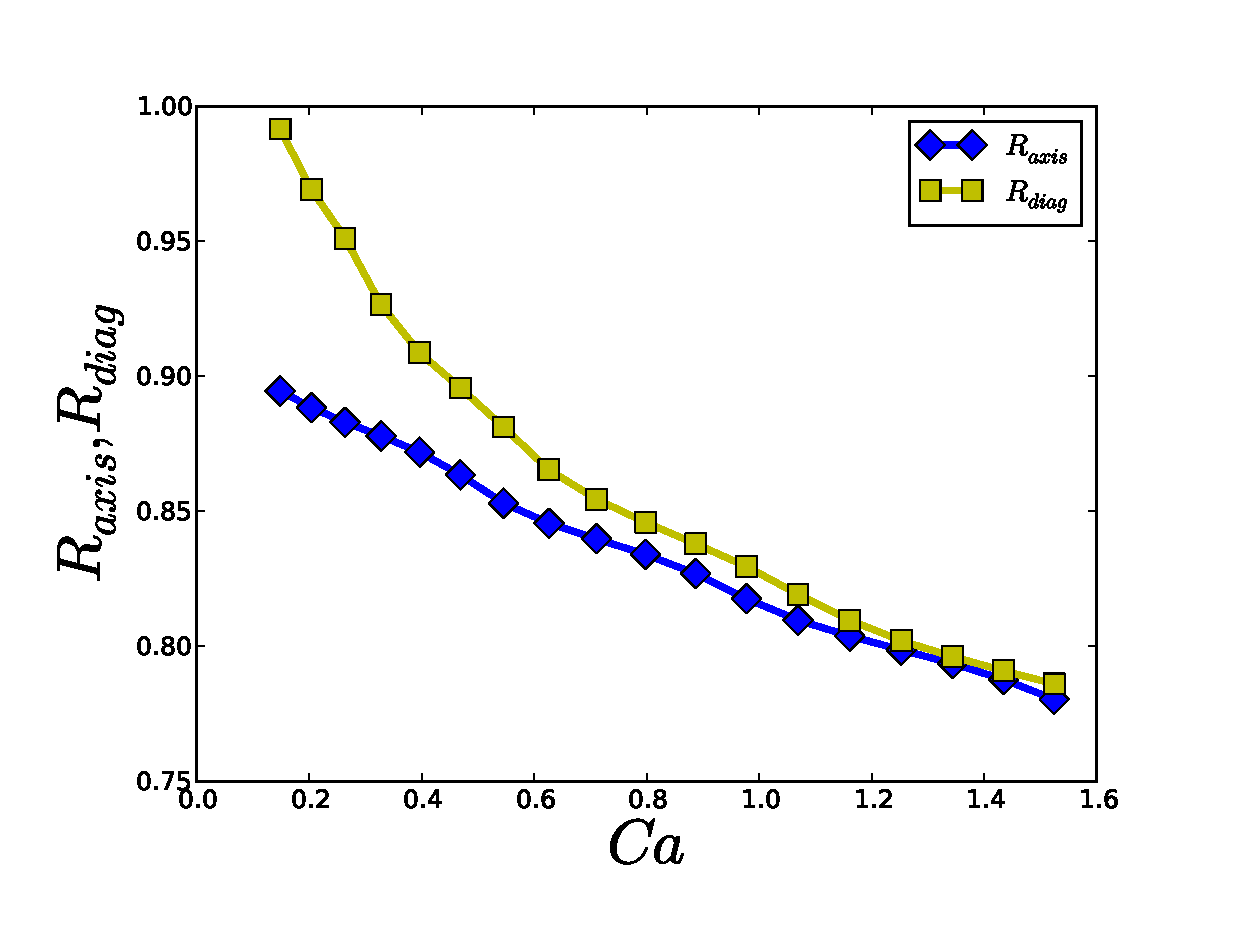
\includegraphics[width=0.97\textwidth]{Figures/underresolved_capillaries.eps}
\caption{The underresolved profiles axis and diagonal radiuses versus capillary numbers. $50$
percent resolution starts from $Ca=1.0$, which is quite high. One can see it's exactly where
radiuses converge instead of $Ca=0.04$. However, one can see from simulations Fig.
\ref{fig:wang:critical:capillary} and Fig.\ref{fig:thickness:variation:ca:ten} the thickness,
especially for Fig.\ref{fig:thickness:variation:ca:ten}, can significantly variate over a bubble
length. \label{fig:underresolved:capillaries}}
\end{figure}

One can see the variation of thickness over the bubble length for the given capillary $Ca=1.06$ in
Fig. \ref{fig:variation:bubble:ca:one}. One can see that variation over the length can be neglected
for relatively high $Ca$ numbers.
\begin{figure}
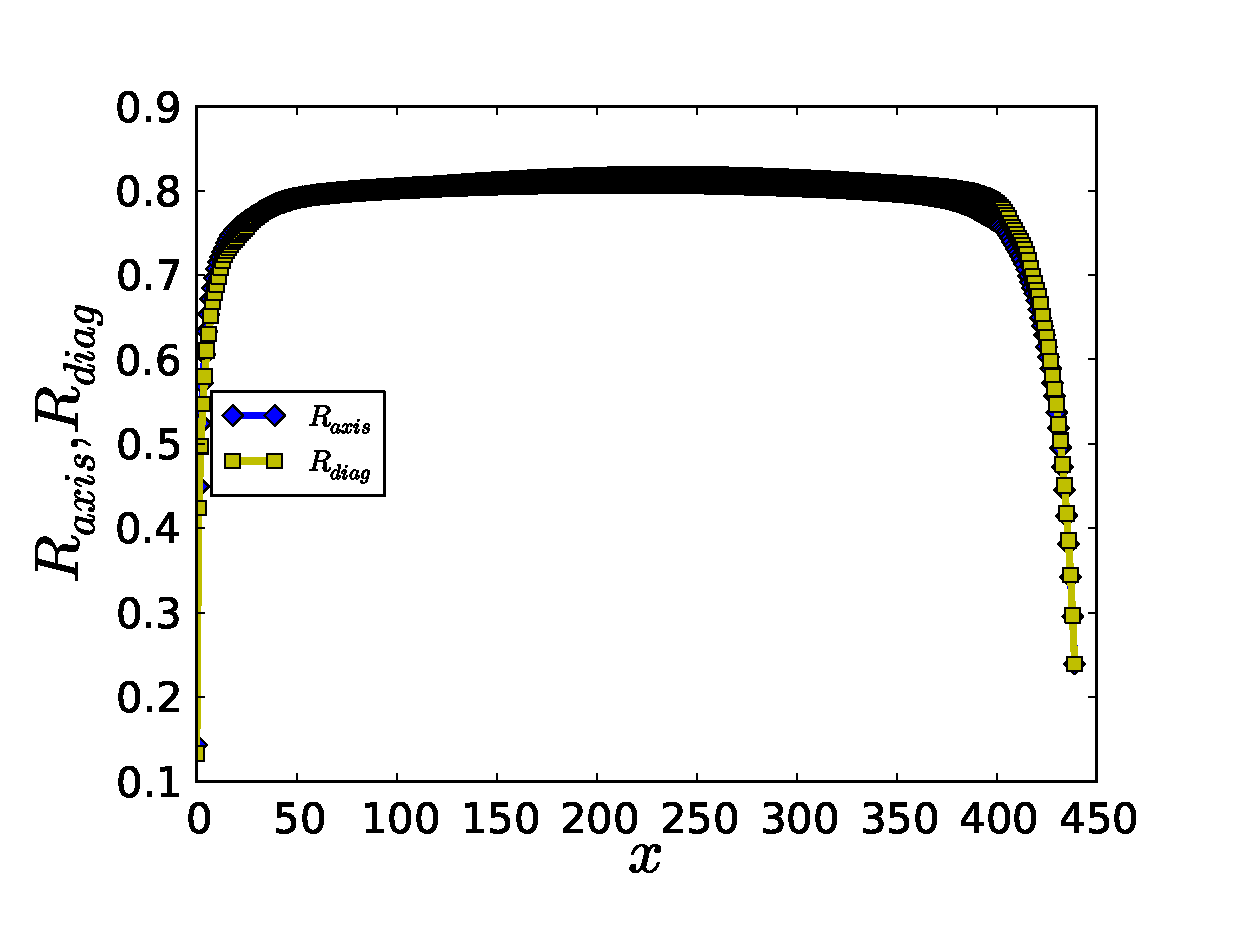
\includegraphics[width=0.97\textwidth]{Figures/bubble_length_ca_one.eps}
\caption{The bubble length variation over for given $Ca=1.06$.
One can see that there is no such high variation over the bubble
length. \label{fig:variation:bubble:ca:one}}
\end{figure}


\section{Steady-state case}
We performed different simulations to understand a number of steps required for the problem to come
on the steady-state. The grid to be simulated is $52\mathrm{x}52\mathrm{x}750$ with the initial
width as $6.5$ lattice Boltzmann units together with $\frac{\mathrm{d}P}{\mathrm{d}x}=3
\mathrm{x}10^{-5}$. The simulation was performed for $200000$,$400000$,$600000$ and $800000$ time
iterations. The results are summarised in Table \ref{table:steady:state}. One of the profiles in
the middle of the bubble is shown in Fig. \ref{fig:steady:state:profile:example}.
\begin{table}
\begin{tabular}{|c|c|c|c|}
$N_{iter}$&$Ca$&$R_{axis}$&$R_{diag}$\\
$200000$&$0.285$&$0.873$&$0.921$\\
$400000$&$0.274$&$0.873$&$0.920$\\
$600000$&$0.263$&$0.872$&$0.919$\\
$800000$&$0.252$&$0.873$&$0.917$\\
\end{tabular}
\caption{Results for the steady-state case. One can see that $200000$ steps are enough to structure
the bubble. However, the interface is underresolved. That could be the influence of the bubble
length.\label{table:steady:state}}
\end{table}
\begin{figure}
\includegraphics[width=0.47\textwidth]{Figures/bullet.eps}\hfill
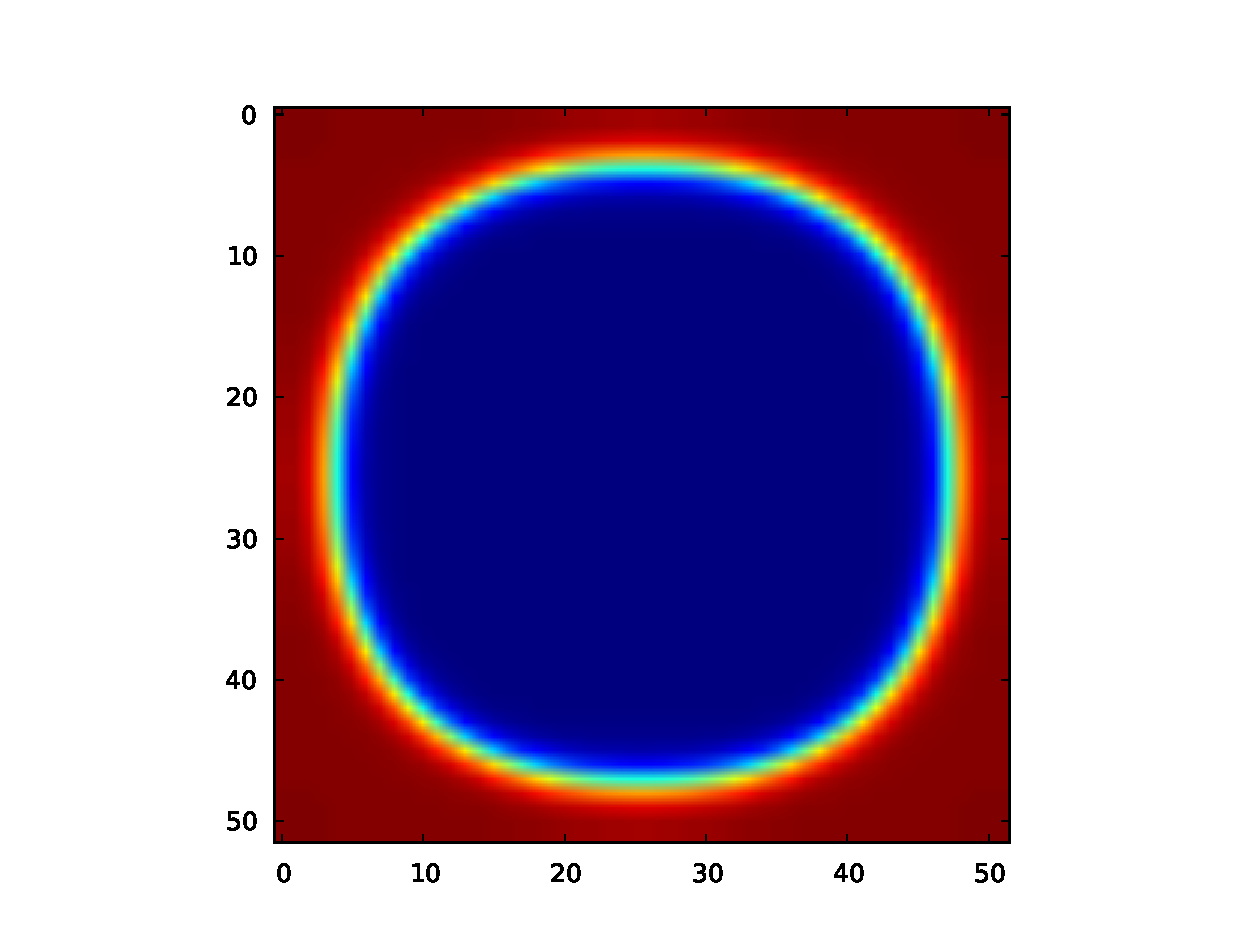
\includegraphics[width=0.47\textwidth]{Figures/example_crossection.eps}\\
\caption{Slice in the middle of the bubble and
three-dimensional example. \label{fig:steady:state:profile:example}}
\end{figure}


To understand the influence of the steady-state case
For the steady-state regime the following parameters were obtained
We want to perform understanding of the steady state regime. As well probably it's good idea to
change domain as well, to reduce the length but to insure enough length of the bubble. The
steady-state calculations are performed on $52\mathrm{x}52\mathrm{x}750$ with large enough the
interface. 

\section{Capillary number region}
The same as in the previous example can help us to identify the necessary capillary regime. The
most important thing is to establish different accentricity factors.

\section{Train simulation}
As far as the requirements for the grid are ``heavy'' we performed a bunch of simulations to
examine how the distance between bubbles influences on the thickness. For this purpose the
simulation was conducted on the grid 82x82x750. We examined different initialized distances between
bubbles. The initial lengths of bubbles were chosen as $300$, $350$, $400$, $450$, $500$, $550$
lattice units. Therefore, the corresponding initial distances between bubbles are
$450$,$400$,$350$,$300$,$250$ lattice units. On the steady state regime the distances become $386$,
$317$, $248$,$176$,$99$,$23$ lattice units. The corresponding capillary numbers calculated based on
the center bubble velocity are as follows $0.905$, $0.986$,$1.08$,$1.19$, $1.33$, $1.49$. The
calculated radiuses (diagonal radius equal to the axes radius) are as follows
$0.783$,$0.778$,$0.772$,$0.764$,$0.753$,$0.747$. Thus, one can see the great impact of the bubbles
on each other velocity for the given body force. However, in terms of the film thicknesses those
numbers look adequate. One can see the film thicknesses dependency on the capillary number for the
\citeauthor{heil-threedim} and bubble train simulations data in Fig. \ref{fig:capillaries:train}. 
\begin{figure}
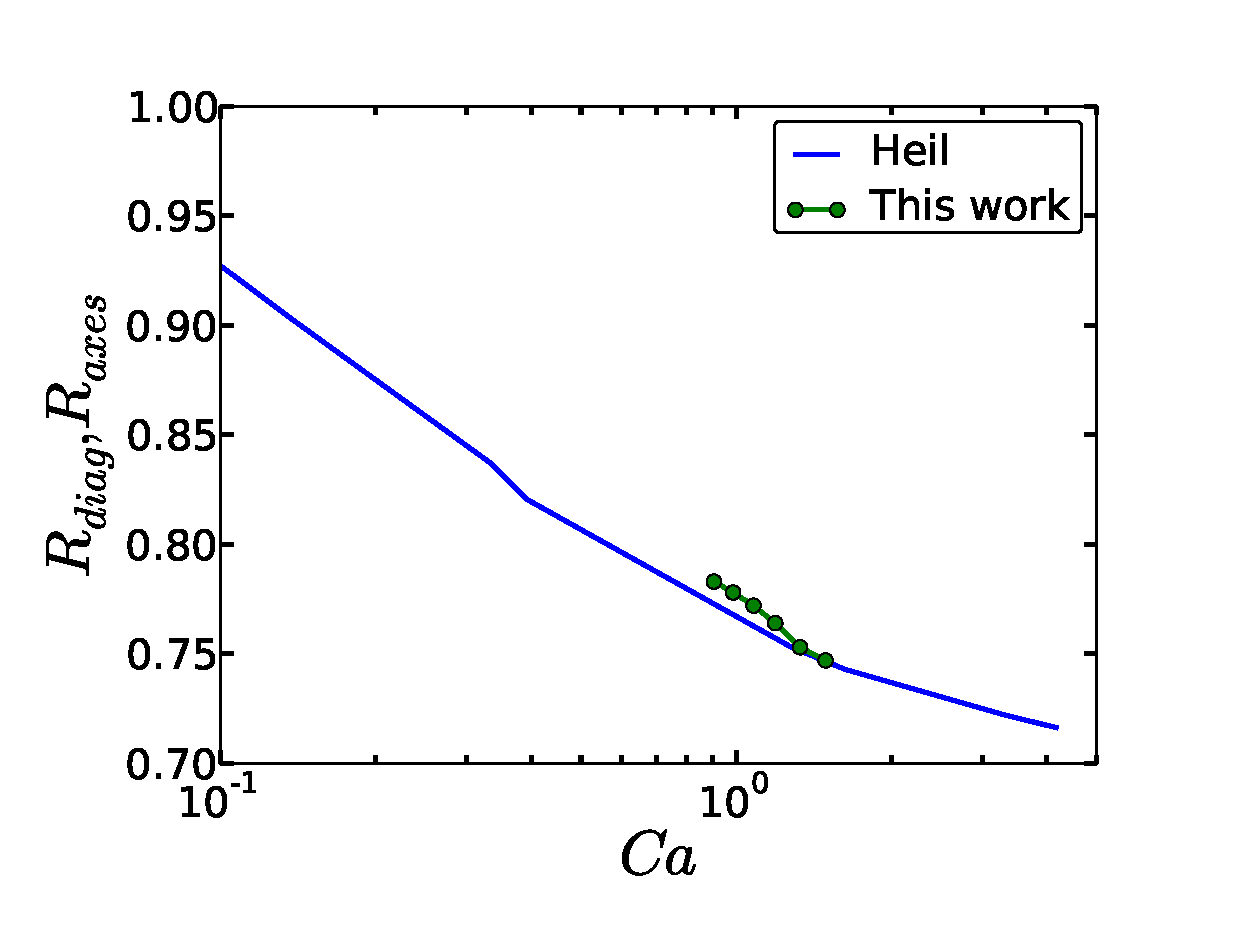
\includegraphics[width=0.97\textwidth]{Figures/capillaries_comparison_train.eps}
\caption{Some more information on representing \label{fig:capillaries:train}}
\end{figure}



\section{Simulation setup}


\bibliographystyle{unsrtnat}
\bibliography{paper}
\end{document}


